%========================================
% EXERCISES: Funciones
%========================================

\section{Ejercicios}

%========================================
% Exercise 1: Identifying Functions
%========================================
\begin{exercise}
Determine si cada relación es una función. Justifique su respuesta.

\problem $\{(2,5), (3,7), (4,5), (5,9)\}$
\begin{solucion}
\textbf{Sí es función.} Cada valor de entrada (2, 3, 4, 5) tiene exactamente una salida. Note que 2 y 4 tienen la misma salida (5), pero esto es permitido.
\end{solucion}

\problem $\{(-1,3), (0,5), (-1,7), (2,9)\}$
\begin{solucion}
\textbf{No es función.} El valor de entrada $-1$ tiene dos salidas diferentes: 3 y 7.
\end{solucion}

\problem $\{(a,1), (b,2), (c,3), (d,4)\}$
\begin{solucion}
\textbf{Sí es función.} Cada letra (valor de entrada) tiene exactamente una salida numérica.
\end{solucion}
\end{exercise}

%========================================
% Exercise 2: Function Evaluation
%========================================
\begin{exercise}
Dada la función $f(x) = 3x^2 - 2x + 1$, evalúe:

\problem $f(2)$
\begin{solucion}
\begin{align*}
f(2) &= 3(2)^2 - 2(2) + 1\\
&= 3(4) - 4 + 1\\
&= 12 - 4 + 1\\
&= 9
\end{align*}
\end{solucion}

\problem $f(-1)$
\begin{solucion}
\begin{align*}
f(-1) &= 3(-1)^2 - 2(-1) + 1\\
&= 3(1) + 2 + 1\\
&= 3 + 2 + 1\\
&= 6
\end{align*}
\end{solucion}

\problem $f(0)$
\begin{solucion}
\begin{align*}
f(0) &= 3(0)^2 - 2(0) + 1\\
&= 0 - 0 + 1\\
&= 1
\end{align*}
\end{solucion}

\problem $f(a-1)$
\begin{solucion}
\begin{align*}
f(a-1) &= 3(a-1)^2 - 2(a-1) + 1\\
&= 3(a^2 - 2a + 1) - 2a + 2 + 1\\
&= 3a^2 - 6a + 3 - 2a + 2 + 1\\
&= 3a^2 - 8a + 6
\end{align*}
\end{solucion}
\end{exercise}

%========================================
% Exercise 3: Linear Function Graphing
%========================================
\begin{exercise}
Dada la función lineal $f(x) = 2x - 3$:

\problem Evalúe la función para $x = -1$, $x = 0$, $x = 1$, y $x = 2$.
\begin{solucion}
\begin{align*}
f(-1) &= 2(-1) - 3 = -2 - 3 = -5\\
f(0) &= 2(0) - 3 = 0 - 3 = -3\\
f(1) &= 2(1) - 3 = 2 - 3 = -1\\
f(2) &= 2(2) - 3 = 4 - 3 = 1
\end{align*}
\end{solucion}

\problem Interprete cada resultado del problema anterior como un punto $(x, y)$ en el plano cartesiano.
\begin{solucion}
Los puntos son:
\begin{itemize}[itemsep=2pt]
    \item $f(-1) = -5$ corresponde al punto $(-1, -5)$
    \item $f(0) = -3$ corresponde al punto $(0, -3)$
    \item $f(1) = -1$ corresponde al punto $(1, -1)$
    \item $f(2) = 1$ corresponde al punto $(2, 1)$
\end{itemize}
\end{solucion}

\problem Ubique los cuatro puntos en el plano cartesiano y trace la gráfica de la función.
\begin{solucion}
\begin{center}
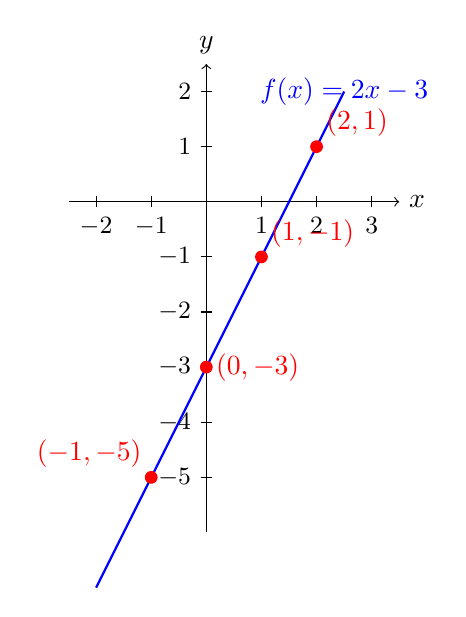
\begin{tikzpicture}[scale=0.7]
    % Axes
    \draw[->] (-2.5,0) -- (3.5,0) node[right] {$x$};
    \draw[->] (0,-6) -- (0,2.5) node[above] {$y$};

    % Grid
    \foreach \x in {-2,-1,1,2,3}
        \draw (\x,0.1) -- (\x,-0.1) node[below] {\small $\x$};
    \foreach \y in {-5,-4,-3,-2,-1,1,2}
        \draw (0.1,\y) -- (-0.1,\y) node[left] {\small $\y$};

    % Plot the line
    \draw[domain=-2:2.5, smooth, blue, thick] plot (\x, {2*\x - 3});

    % Plot the points
    \filldraw[red] (-1,-5) circle (3pt);
    \filldraw[red] (0,-3) circle (3pt);
    \filldraw[red] (1,-1) circle (3pt);
    \filldraw[red] (2,1) circle (3pt);

    % Labels for points
    \node[red, above left] at (-1,-5) {$(-1,-5)$};
    \node[red, right] at (0,-3) {$(0,-3)$};
    \node[red, above right] at (1,-1) {$(1,-1)$};
    \node[red, above right] at (2,1) {$(2,1)$};

    % Function label
    \node[blue] at (2.5,2) {$f(x) = 2x - 3$};
\end{tikzpicture}
\end{center}

\textbf{Observación:} Todos los puntos están alineados formando una recta. Esto confirma que $f(x) = 2x - 3$ es una función lineal con:
\begin{itemize}[itemsep=2pt]
    \item Pendiente $m = 2$ (sube 2 unidades por cada unidad a la derecha)
    \item Intercepto en $y$: $(0, -3)$
\end{itemize}
\end{solucion}
\end{exercise}

%========================================
% Exercise 4: Domain
%========================================
\begin{exercise}
Encuentre el dominio de cada función:

\problem $f(x) = \dfrac{1}{x+5}$
\begin{solucion}
El denominador no puede ser cero: $x + 5 \ne 0 \Rightarrow x \ne -5$

\textbf{Dominio:} $(-\infty, -5) \cup (-5, \infty)$ o ``todos los reales excepto $-5$''
\end{solucion}

\problem $g(x) = \sqrt{x-7}$
\begin{solucion}
Para raíces cuadradas, el radicando debe ser no negativo:
\begin{align*}
x - 7 &\ge 0\\
x &\ge 7
\end{align*}

\textbf{Dominio:} $[7, \infty)$
\end{solucion}

\problem $h(x) = \dfrac{\sqrt{x-5}}{x-7}$
\begin{solucion}
Necesitamos dos condiciones:
\begin{itemize}
    \item Radicando no negativo: $x - 5 \ge 0 \Rightarrow x \ge 5$
    \item Denominador no cero: $x - 7 \ne 0 \Rightarrow x \ne 7$
\end{itemize}

Combinando: $x \ge 5$ pero $x \ne 7$

\textbf{Dominio:} $[5, 7) \cup (7, \infty)$
\end{solucion}

\problem $k(x) = 5x - 3$
\begin{solucion}
Esta es una función lineal sin restricciones.

\textbf{Dominio:} $(-\infty, \infty)$ o ``todos los números reales''
\end{solucion}
\end{exercise}

%========================================
% Exercise 5: Mixed Problems
%========================================
\begin{exercise}
Problemas variados:

\problem ¿La gráfica de $x^2 + y^2 = 16$ representa una función? Use la prueba de la recta vertical.
\begin{solucion}
\textbf{No.} Esta ecuación representa un círculo con centro en el origen y radio 4.

Si trazamos una recta vertical, por ejemplo $x = 0$, interseca el círculo en dos puntos: $(0, 4)$ y $(0, -4)$.

Por la prueba de la recta vertical, como existe al menos una recta vertical que interseca la gráfica en más de un punto, la relación \textbf{no es función}.
\end{solucion}

\problem Dada $f(x) = |x + 2|$, identifique:
\begin{exerciselist}
    \item El vértice de la gráfica
    \item El dominio
    \item El rango
\end{exerciselist}
\begin{solucion}
\begin{exerciselist}
    \item \textbf{Vértice:} $(-2, 0)$ (la expresión dentro del valor absoluto se hace cero cuando $x = -2$)
    \item \textbf{Dominio:} $(-\infty, \infty)$ (todas las funciones de valor absoluto tienen dominio de todos los reales)
    \item \textbf{Rango:} $[0, \infty)$ (el valor absoluto siempre produce valores no negativos)
\end{exerciselist}
\end{solucion}

\problem ¿Cuál es el dominio de $f(x) = \sqrt{x+3}$? Grafique la función indicando el punto inicial.
\begin{solucion}
\textbf{Dominio:} Necesitamos $x + 3 \ge 0 \Rightarrow x \ge -3$, entonces el dominio es $[-3, \infty)$

\textbf{Gráfica:}
\begin{center}
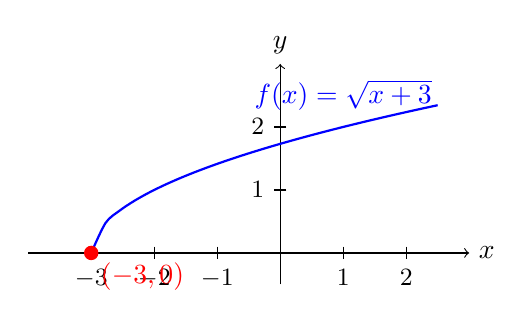
\begin{tikzpicture}[scale=0.8]
    \draw[->] (-4,0) -- (3,0) node[right] {$x$};
    \draw[->] (0,-0.5) -- (0,3) node[above] {$y$};

    % Grid
    \foreach \x in {-3,-2,-1,1,2}
        \draw (\x,0.1) -- (\x,-0.1) node[below] {\small $\x$};
    \foreach \y in {1,2}
        \draw (0.1,\y) -- (-0.1,\y) node[left] {\small $\y$};

    % Function
    \draw[domain=-3:2.5, smooth, blue, thick] plot (\x, {sqrt(\x+3)});

    % Starting point
    \filldraw[red] (-3,0) circle (3pt);
    \node[red, below right] at (-3,0) {$(-3,0)$};

    \node[blue] at (1,2.5) {$f(x) = \sqrt{x+3}$};
\end{tikzpicture}
\end{center}

La función empieza en $(-3, 0)$ y crece hacia la derecha.
\end{solucion}

\problem Para $g(x) = x^2 - 4$, encuentre:
\begin{exerciselist}
    \item $g(3)$
    \item Los valores de $x$ donde $g(x) = 0$ (ceros de la función)
    \item El vértice de la parábola
\end{exerciselist}
\begin{solucion}
\begin{exerciselist}
    \item $g(3) = (3)^2 - 4 = 9 - 4 = 5$

    \item Para encontrar los ceros, resolvemos $g(x) = 0$:
    \begin{align*}
    x^2 - 4 &= 0\\
    (x-2)(x+2) &= 0\\
    x &= 2 \text{ o } x = -2
    \end{align*}
    Los ceros son $x = -2$ y $x = 2$

    \item Para $f(x) = ax^2 + bx + c$, el vértice está en $x = -\dfrac{b}{2a}$

    En este caso: $a = 1$, $b = 0$, $c = -4$
    $$x = -\frac{0}{2(1)} = 0$$

    El valor de $y$ es: $g(0) = 0^2 - 4 = -4$

    \textbf{Vértice:} $(0, -4)$
\end{exerciselist}
\end{solucion}
\end{exercise}
